\documentclass[10pt,mathserif]{beamer}

\usepackage{graphicx,amsmath,amssymb,psfrag,mathtools}
\usepackage{soul}
\usepackage{amsmath,amsfonts,amsthm,bbm}
\usepackage{stmaryrd}
\usepackage{subcaption}



%Code block environment
\usepackage{listings}


\definecolor{lightgrey}{gray}{0.8}
\definecolor{medgrey}{gray}{0.6}
\definecolor{darkgrey}{gray}{0.4}
\usepackage{xcolor}
\lstset { %
    backgroundcolor=\color{black!5}, % set backgroundcolor
    basicstyle=\ttfamily,
    showstringspaces=false,
    commentstyle = \ttfamily,
    commentstyle=\color{commentgreen}\ttfamily,
    morecomment=[l][\color{darkgrey}]{//},
}



\usepackage{tikz}
\usetikzlibrary{matrix,chains,positioning,decorations.pathreplacing,arrows}
\usetikzlibrary{positioning,calc}
\usepackage{tkz-euclide}
%\usetkzobj{all}





%-------------------------------------------------------------------------------
%Definition of operator font
 \usepackage[bb=boondox]{mathalfa}
%% import \varmathbb without affecting other fonts
\usepackage{xparse}
\DeclareFontFamily{U}{ntxmia}{}
\DeclareFontShape{U}{ntxmia}{m}{it}{<-> ntxmia }{}
\DeclareFontShape{U}{ntxmia}{b}{it}{<-> ntxbmia }{}
\DeclareSymbolFont{lettersA}{U}{ntxmia}{m}{it}
\SetSymbolFont{lettersA}{bold}{U}{ntxmia}{b}{it}
\ExplSyntaxOn
\NewDocumentCommand{\varmathbb}{m}
 {
  \tl_map_inline:nn { #1 }
   {
    \use:c { varbb##1 }
   }
 }
\tl_map_inline:nn { ABCDEFGHIJKLMNOPQRSTUVWXYZ }
 {
  \exp_args:Nc \DeclareMathSymbol{varbb#1}{\mathord}{lettersA}{\int_eval:n { `#1+67 }}
 }
\exp_args:Nc \DeclareMathSymbol{varbbk}{\mathord}{lettersA}{169}
\ExplSyntaxOff
%%
\makeatletter
\DeclareFontFamily{U}{tipa}{}
\DeclareFontShape{U}{tipa}{m}{n}{<->tipa10}{}
\newcommand{\arc@char}{{\usefont{U}{tipa}{m}{n}\symbol{62}}}%

\newcommand{\arc}[1]{\mathpalette\arc@arc{#1}}

\newcommand{\arc@arc}[2]{%
  \sbox0{$\m@th#1#2$}%
  \vbox{
    \hbox{\resizebox{\wd0}{\height}{\arc@char}}
    \nointerlineskip
    \box0
  }%
}
\makeatother
\newcommand{\opA}{{\varmathbb{A}}}
\newcommand{\opB}{{\varmathbb{B}}}
\newcommand{\opC}{{\varmathbb{C}}}
\newcommand{\opD}{{\varmathbb{D}}}
\newcommand{\opE}{{\varmathbb{E}}}
\newcommand{\opF}{{\varmathbb{F}}}
\newcommand{\opG}{{\varmathbb{G}}}
\newcommand{\opH}{{\varmathbb{H}}}
\newcommand{\opI}{{\varmathbb{I}}}
\newcommand{\opJ}{{\varmathbb{J}}}
\newcommand{\opK}{{\varmathbb{K}}}
\newcommand{\opL}{{\varmathbb{L}}}
\newcommand{\opM}{{\varmathbb{M}}}
\newcommand{\opN}{{\varmathbb{N}}}
\newcommand{\opO}{{\varmathbb{O}}}
\newcommand{\opP}{{\varmathbb{P}}}
\newcommand{\opQ}{{\varmathbb{Q}}}
\newcommand{\opR}{{\varmathbb{R}}}
\newcommand{\opS}{{\varmathbb{S}}}
\newcommand{\opT}{{\varmathbb{T}}}
\newcommand{\opU}{{\varmathbb{U}}}
\newcommand{\opV}{{\varmathbb{V}}}
\newcommand{\opW}{{\varmathbb{W}}}
\newcommand{\opX}{{\varmathbb{X}}}
\newcommand{\opY}{{\varmathbb{Y}}}
\newcommand{\opZ}{{\varmathbb{Z}}}
\newcommand{\opZer}{\mathbb{0}}
%-------------------------------------------------------------------------------



%-------------------------------------------------------------------------------
%Definition of other font types
\newcommand{\va}{{\mathbf{a}}}
\newcommand{\vb}{{\mathbf{b}}}
\newcommand{\vc}{{\mathbf{c}}}
\newcommand{\vd}{{\mathbf{d}}}
\newcommand{\ve}{{\mathbf{e}}}
\newcommand{\vf}{{\mathbf{f}}}
\newcommand{\vg}{{\mathbf{g}}}
\newcommand{\vh}{{\mathbf{h}}}
\newcommand{\vi}{{\mathbf{i}}}
\newcommand{\vj}{{\mathbf{j}}}
\newcommand{\vk}{{\mathbf{k}}}
\newcommand{\vl}{{\mathbf{l}}}
\newcommand{\vm}{{\mathbf{m}}}
\newcommand{\vn}{{\mathbf{n}}}
\newcommand{\vo}{{\mathbf{o}}}
\newcommand{\vp}{{\mathbf{p}}}
\newcommand{\vq}{{\mathbf{q}}}
\newcommand{\vr}{{\mathbf{r}}}
\newcommand{\vs}{{\mathbf{s}}}
\newcommand{\vt}{{\mathbf{t}}}
\newcommand{\vu}{{\mathbf{u}}}
\newcommand{\vv}{{\mathbf{v}}}
\newcommand{\vw}{{\mathbf{w}}}
\newcommand{\vx}{{\mathbf{x}}}
\newcommand{\vy}{{\mathbf{y}}}
\newcommand{\vz}{{\mathbf{z}}}

\newcommand{\vA}{{\mathbf{A}}}
\newcommand{\vB}{{\mathbf{B}}}
\newcommand{\vC}{{\mathbf{C}}}
\newcommand{\vD}{{\mathbf{D}}}
\newcommand{\vE}{{\mathbf{E}}}
\newcommand{\vF}{{\mathbf{F}}}
\newcommand{\vG}{{\mathbf{G}}}
\newcommand{\vH}{{\mathbf{H}}}
\newcommand{\vI}{{\mathbf{I}}}
\newcommand{\vJ}{{\mathbf{J}}}
\newcommand{\vK}{{\mathbf{K}}}
\newcommand{\vL}{{\mathbf{L}}}
\newcommand{\vM}{{\mathbf{M}}}
\newcommand{\vN}{{\mathbf{N}}}
\newcommand{\vO}{{\mathbf{O}}}
\newcommand{\vP}{{\mathbf{P}}}
\newcommand{\vQ}{{\mathbf{Q}}}
\newcommand{\vR}{{\mathbf{R}}}
\newcommand{\vS}{{\mathbf{S}}}
\newcommand{\vT}{{\mathbf{T}}}
\newcommand{\vU}{{\mathbf{U}}}
\newcommand{\vV}{{\mathbf{V}}}
\newcommand{\vW}{{\mathbf{W}}}
\newcommand{\vX}{{\mathbf{X}}}
\newcommand{\vY}{{\mathbf{Y}}}
\newcommand{\vZ}{{\mathbf{Z}}}

\newcommand{\cA}{{\mathcal{A}}}
\newcommand{\cB}{{\mathcal{B}}}
\newcommand{\cC}{{\mathcal{C}}}
\newcommand{\cD}{{\mathcal{D}}}
\newcommand{\cE}{{\mathcal{E}}}
\newcommand{\cF}{{\mathcal{F}}}
\newcommand{\cG}{{\mathcal{G}}}
\newcommand{\cH}{{\mathcal{H}}}
\newcommand{\cI}{{\mathcal{I}}}
\newcommand{\cJ}{{\mathcal{J}}}
\newcommand{\cK}{{\mathcal{K}}}
\newcommand{\cL}{{\mathcal{L}}}
\newcommand{\cM}{{\mathcal{M}}}
\newcommand{\cN}{{\mathcal{N}}}
\newcommand{\cO}{{\mathcal{O}}}
\newcommand{\cP}{{\mathcal{P}}}
\newcommand{\cQ}{{\mathcal{Q}}}
\newcommand{\cR}{{\mathcal{R}}}
\newcommand{\cS}{{\mathcal{S}}}
\newcommand{\cT}{{\mathcal{T}}}
\newcommand{\cU}{{\mathcal{U}}}
\newcommand{\cV}{{\mathcal{V}}}
\newcommand{\cW}{{\mathcal{W}}}
\newcommand{\cX}{{\mathcal{X}}}
\newcommand{\cY}{{\mathcal{Y}}}
\newcommand{\cZ}{{\mathcal{Z}}}
%-------------------------------------------------------------------------------




%-------------------------------------------------------------------------------
%% macros for math notions and operators
\newcommand{\EE}{{\mathbb{E}}}
\newcommand{\expec}{\mathbb{E}}
\newcommand{\Prob}{{\mathrm{Prob}}} % probability

\newcommand{\reals}{\mathbb{R}}
\newcommand{\RR}{\mathbb{R}}
\newcommand{\complex}{\mathbb{C}}
\newcommand{\CC}{\mathbb{C}}
\newcommand{\nats}{\mathbb{N}}
\newcommand{\NN}{\mathbb{N}}
\newcommand{\ZZ}{\mathbb{Z}}
\newcommand{\bigO}{\mathcal{O}}
\newcommand{\order}[1]{{\mathcal{O}\left(#1\right)}}
\renewcommand{\SS}{{\mathbb{S}}}
\newcommand{\SSp}{\mathbb{S}_{+}}
\newcommand{\SSpp}{\mathbb{S}_{++}}
\newcommand{\sign}{\mathrm{sign}}
\newcommand{\vzero}{\mathbf{0}}
\newcommand{\vone}{{\mathbf{1}}}

\renewcommand{\Re}{\operatorname{Re}} 	%Real part
\renewcommand{\Im}{\operatorname{Im}}	%imaginary part

%\newcommand{\supp}{{\mathrm{supp}}} % support
\newcommand{\range}{\mathrm{range}\,} % domain
\newcommand{\tr}{{\mathrm{tr}}} % trace
%-------------------------------------------------------------------------------





%-------------------------------------------------------------------------------
%% Theorem definitions
\setbeamertemplate{theorems}[ams style] 
\newtheorem*{theorem*}{Theorem}
%\newtheorem{lemma}{Lemma}    % already provided by amsthm
\newtheorem{proposition}{Proposition}
%\newtheorem{proof}{Proof}  % already provided by amsthm


%-------------------------------------------------------------------------------
%% operator and convex analysis definitions

\newcommand*{\fix}{\mathrm{Fix}\,}
\newcommand*{\zer}{\mathrm{Zer}\,}
\newcommand*{\gra}{\mathrm{Gra}\,}
\newcommand{\prox}{\mathrm{Prox}}
\newcommand{\proj}{\Pi}
\newcommand{\aff}{\mathrm{aff}\,}    %affine hull
\newcommand{\intr}{\mathrm{int}\,}   %interior
\newcommand{\relint}{\mathrm{ri}\,}  %relative interior
\newcommand{\dom}{\mathrm{dom}\,} % domain
\newcommand{\epi}{\mathrm{epi}\,} % epigraph
\newcommand{\dist}{\mathrm{dist}}
\newcommand{\lagrange}{\mathbf{L}}  %saddle function
\newcommand{\fitzpatrick}{\mathbf{F}}   %Fitzpatrick function
\newcommand{\vecdelay}{\boldsymbol{d}}   %vector delay
\DeclareMathOperator*{\argmin}{argmin}
\DeclareMathOperator*{\argmax}{argmax}

%-------------------------------------------------------------------------------
%SRG definitions
\newcommand{\ereal}{\overline{\mathbb{R}^2}}
\newcommand{\ecomplex}{\overline{\mathbb{C}}}
\newcommand{\binfty}{{\boldsymbol \infty}}
\newcommand{\rarc}{\mathrm{Arc}^+}
\newcommand{\larc}{\mathrm{Arc}^-}


%-------------------------------------------------------------------------------




%-------------------------------------------------------------------------------
%Miscellaneous Stuff
%% sequences
\newcommand{\itom}{_{i=1}^{m}}
\newcommand{\ieqm}{i=1,\dots,m}

% use \numberthis to add an equation number in align*
\newcommand\numberthis{\addtocounter{equation}{1}\tag{\theequation}}

\newcolumntype{P}[1]{>{\centering\arraybackslash}p{#1}}

\mode<presentation>
{
\usetheme{default}
}
\setbeamertemplate{navigation symbols}{}
\usecolortheme[rgb={0.13,0.28,0.59}]{structure}
\setbeamertemplate{itemize subitem}{--}
\setbeamertemplate{frametitle} {
	\begin{center}
	  {\large\bf \insertframetitle}
	\end{center}
}

\newcommand\footlineon{
  \setbeamertemplate{footline} {
    \begin{beamercolorbox}[ht=2.5ex,dp=1.125ex,leftskip=.8cm,rightskip=.6cm]{structure}
      \footnotesize \insertsection
      \hfill
      {\insertframenumber}
    \end{beamercolorbox}
    \vskip 0.45cm
  }
}
\footlineon


\newcommand\footlineoff{
  \setbeamertemplate{footline} {
    \begin{beamercolorbox}[ht=2.5ex,dp=1.125ex,leftskip=.8cm,rightskip=.6cm]{structure}
      \footnotesize 
      \hfill
      {\insertframenumber}
    \end{beamercolorbox}
    \vskip 0.45cm
  }
}


\newcommand\blfootnote[1]{%
  \begingroup
  \renewcommand\thefootnote{}\footnote{#1}%
  \addtocounter{footnote}{-1}%
  \endgroup
}


\AtBeginSection[] 
{ 
	\begin{frame}<beamer> 
		\frametitle{Outline} 
		\tableofcontents[currentsection,currentsubsection] 
	\end{frame} 
} 

%% wotao's preference

        % itemize, black bullet, %150 spacing between items using "witemize"
        \newenvironment{witemize}{\itemize\addtolength{\itemsep}{0.3\baselineskip}}{\enditemize}

\iffalse
        % \setbeamertemplate{itemize items}[square]
        \setbeamertemplate{itemize items}{\textbullet}
        \setbeamercolor{itemize item}{fg=black}
        \setbeamercolor{itemize subitem}{fg=black}
        \setbeamercolor{itemize subsubitem}{fg=black}
        \setbeamercolor{enumerate item}{fg=black}
        \setbeamercolor{enumerate subitem}{fg=black}
        \setbeamercolor{enumerate subsubitem}{fg=black}
        \setbeamertemplate{itemize/enumerate body begin}{\normalsize}
        \setbeamertemplate{itemize/enumerate subbody begin}{\normalsize}
        \setbeamertemplate{itemize/enumerate subsubbody begin}{\normalsize}

        % itemize enumerate use normal sized texts
        \setbeamertemplate{itemize/enumerate body begin}{\normalsize}
        \setbeamertemplate{itemize/enumerate subbody begin}{\normalsize}
        \setbeamertemplate{itemize/enumerate subsubbody begin}{\normalsize}

        % block, black over gray with no shadow
        \setbeamertemplate{blocks}[rounded][shadow=false]
        \setbeamercolor{block title}{fg=black,bg=gray!40}
        \setbeamercolor{block body}{fg=black,bg=gray!10}
\fi

\author{Ernest K. Ryu and Wotao Yin}

\date{Large-Scale Convex Optimization via Monotone Operators}


\title{\large \bfseries Distributed and Decentralized Optimization}

\begin{document}

\frame{
\thispagestyle{empty}
\titlepage
}

\begin{frame}{Distributed optimization}
    Distributed optimization uses a set of networked computers, called agents, to solve optimization problems.
    \bigskip
    
    \emph{Motivation}: When an algorithm running on one computer does not meet the required performance, one can
    \begin{enumerate}
        \item upgrade the computer (CPU, memory) and run the same algorithm;
        \item use more computers, decompose the problem, and run a distributed optimization algorithm.
    \end{enumerate}
    \pause\smallskip
    
    Approach 1 is less cost effective and may never reach the required performance. 
    \medskip
    
    Approach 2 is the more favorable (often the only) choice of solving extremely large optimization problems.
\end{frame}

\begin{frame}{Decentralized optimization}

    We distinguish between \emph{distributed methods} and \emph{decentralized methods}.
    \pause\medskip
    
    \emph{Distributed methods} perform computation over a network (a broader class). 
    \medskip
    
    \emph{Decentralized methods} do so without central coordination (a subclass).
    \pause\medskip
    
    Roughly speaking, when communication latency and bandwidth cost much more than computation, decentralized methods are preferred.
    \medskip
    
    Examples: drone fleet control, wireless sensor network, applications of real-time decisions made based on agents' local data
\end{frame}

\begin{frame}
\frametitle{Problem and setup}
In this lecture, we solve
\begin{equation}
\begin{array}{ll}
\underset{x\in\reals^p}{\mbox{minimize}} & \displaystyle{\sum_{i=1}^n \left(f_i(x)+h_i(x)\right)},
\end{array}
\label{eq:dist-main-opt}
\end{equation}
where $f_1,\dots,f_n$ are CCP (and proximable) and $h_1,\dots,h_n$ are CCP and differentiable.
\pause\bigskip

\emph{Setup}: agents $i=1,\dots,n$ each perform local computation with $f_i$ and $h_i$ and communicate over a network to find the (shared) solution $x^\star$.
\pause\bigskip

The textbook chapter considers the more general formulation
\begin{equation}
\begin{array}{ll}
\underset{x\in\reals^p}{\mbox{minimize}} & r(x)+\displaystyle{\sum_{i=1}^n \left(f_i(x)+h_i(x)\right)},
\end{array}
\end{equation}
where $r$ is CCP and proximable.

%In this chapter, we study distributed and decentralized methods that allow computational agents communicating over a network to collaboratively solve an optimization problem.

% \vspace{0.2in}
% We distinguish \emph{distributed} and \emph{decentralized} methods: \\
% distributed methods compute over a network (broader class) while decentralized methods do so without central coordination (special case).
% In other words, distributed methods is a broader class of methods that include decentralized methods as special cases.

\end{frame}

% \begin{frame}
% \frametitle{Distributed and decentralized applications}
% One application of distributed optimization is solving extremely large optimization problems that require the computing power of a cluster of computers communicating over a network.

% \vspace{0.2in}
% Another application is controlling a fleet of autonomous vehicles (such as drones) or a wireless sensor network, where individual agents make real-time decisions based on data gathered by itself and other agents.


% \vspace{0.2in}

% Decentralized methods are effective for these setups as they minimize the high cost and latency of communication.
% \end{frame}



\section{Distributed optimization with centralized consensus}
\begin{frame}
\frametitle{Centralized consensus}
Consider a parameter-server network model with a centralized agent coordinating with $n$ individual agents.
%. This network structure allows efficient distributed centralized optimization.

\begin{center}
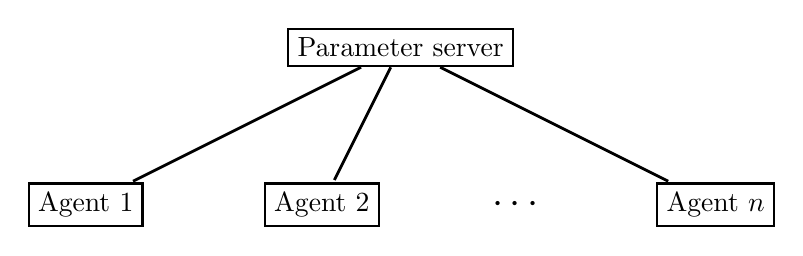
\begin{tikzpicture}
[->,>=stealth',shorten >=1pt,auto,node distance=3cm,
                    thick,main node/.style={draw}]

  \node[main node] (1) at (4, 2) {Parameter server};
  \node[main node] (2) at (0, 0)  {Agent $1$};
  \node[main node] (3) at (3, 0)  {Agent $2$};
  \node[] (5) at (5.5, 0)  {\Large{$\cdots$}};
  \node[main node] (4) at (8, 0)  {Agent $n$};

  \path[line width=1pt,-]
    (1) edge node [left] {} (2)
    (1) edge node [left] {} (3)
    (1) edge node [left] {} (4);
\end{tikzpicture}
\end{center}

\vspace{0.2in}

We study distributed methods based on the consensus technique.
%The relatively simple, centralized communication structure of these methods allow us to analyze them with the tools of we already know.

\end{frame}


\begin{frame}
\frametitle{Distributed gradient method}
Consider 
\[
\begin{array}{ll}
\underset{x\in\reals^p}{\mbox{minimize}} &\displaystyle{\frac{1}{n}\sum_{i=1}^n h_i(x)},
\end{array}
\]
where $h_1,\dots,h_n$ are differentiable.
With consensus set $C=\{(x_1,\dots,x_n)\,|\,x_1=\dots=x_n\}$, obtain the equivalent problem
\[
\begin{array}{ll}
\underset{x_1,\dots,x_n \in\reals^p}{\mbox{minimize}} &\displaystyle{\frac{1}{n}\sum_{i=1}^n h_i(x_i)}\\
\mbox{subject to}& (x_1,\dots,x_n)\in C.
\end{array}
\]
\pause 
FBS is:
\begin{align*}
x^{k+1/2}_i&=x^k-\alpha\nabla h_i(x^k)\\
x^{k+1}&=\frac{1}{n}\sum^n_{i=1}x_i^{k+1/2}
\end{align*}
\end{frame}


\begin{frame}
\frametitle{Distributed gradient method}
Equivalent to:
\begin{align*}
\bar{g}^k&=\frac{1}{n}\sum^n_{i=1}\nabla h_i(x^k)\\
x^{k+1}&=x^{k}-\alpha \bar{g}^k
\end{align*}
This is the distributed gradient method.
Assume a solution exists, $h_1,\dots,h_n$ are $L_h$-smooth, and $\alpha\in (0,2/L_h)$. Then $x^k\rightarrow x^\star$.\\
(When $h_1,\dots,h_n$  not differentiable, can use subgradient method of \S7.)
\pause\vspace{0.2in}

This method is (centralized) distributed: 
%as it has a distributed implementation that alternates local computation and centralized communication in a setup with $n$ computational agents and a central node as in Figure~\ref{figure:centralized_graph}:
\begin{itemize}
\item[(i)] Each agent independently computes $\nabla h_i(x^k)$
\item[(ii)] Agents coordinate to compute $\bar{g}^k$ (reduction operation) and the central agent computes and broadcasts $x^{k+1}$ to all individual agents.
\end{itemize}
%The centralized communication and computation of $g^k$ in step (ii) is called a \emph{reduce} operation in the parallel computing literature.
\end{frame}


\begin{frame}[plain]
\frametitle{Distributed ADMM}
Consider
\[
\begin{array}{ll}
\underset{x\in\reals^p}{\mbox{minimize}} &\displaystyle{\sum_{i=1}^n f_i(x)}.
\end{array}
\]
With the consensus technique, obtain the equivalent problem:
\[
\begin{array}{ll}
\underset{\substack{x_1,\dots,x_n\in\reals^p\\y\in \reals^p}}{\mbox{minimize}} &\displaystyle{\sum_{i=1}^n f_i(x_i)}\\
\mbox{subject to}& x_i=y\qquad\text{for } i=1,\dots,n.
\end{array}
\]
Rewrite to fit ADMM's form:
\[
\begin{array}{ll}
\underset{\substack{x_1,\dots,x_n\in \reals^p\\y\in \reals^p}}{\mbox{minimize}} &\displaystyle{\sum_{i=1}^n f_i(x_i)}\\
\mbox{subject to}&
\begin{bmatrix}
I&0&\cdots&0\\
\vdots&\ddots&&\vdots\\
0&0&\cdots&I\\
\end{bmatrix}\
\begin{bmatrix}
x_1\\\vdots\\x_n
\end{bmatrix}
+
\begin{bmatrix}
-I\\
\vdots\\
-I
\end{bmatrix}
y
=0.
\end{array}
\]
\end{frame}


\begin{frame}
% \frametitle{Distributed ADMM}
Apply ADMM:
\begin{align*}
x_i^{k+1}&=\argmin_{x_i\in \reals^p}\left\{f_i(x_i)+\langle u^k_i,x_i-y^k\rangle+\frac{\alpha}{2}\|x_i-y^k\|^2\right\}\\
y^{k+1}&=\frac{1}{n}\sum^n_{i=1}\left(x_i^{k+1}+\frac{1}{\alpha}u_i^k\right)\\
u_i^{k+1}&=u^k_i+\alpha(x_i^{k+1}-y^{k+1}).
\end{align*}
Simplify the iteration by noting that $u^k_1,\dots,u^k_n$ has mean $0$ after the initial iteration and eliminating $y^k$:
\begin{align*}
%x_i^{k+1}&=\argmin_{x_i}\left\{f_i(x_i)+\langle u^k_i,x_i-\bar{x}^{k}\rangle+\frac{\alpha}{2}\|x_i-\bar{x}^{k}\|^2\right\}\label{eq:distributedADMM1}\\
x_i^{k+1}&=\prox_{(1/\alpha)f_i}\left(\bar{x}^{k}-(1/\alpha)u^k_i\right)\\
%\bar{x}^{k+1}&=\frac{1}{n}\sum^n_{i=1}x_i^{k+1}\\
u_i^{k+1}&=u^k_i+\alpha(x_i^{k+1}-\bar{x}^{k+1})
\end{align*}
for $i=1,\dots,n$,
where $\bar{x}^{k}=(1/n)(x_1^k+\dots+x_n^k)$.
This is distributed (centralized) ADMM.
Convergence follows from convergence of ADMM.
\end{frame}




\begin{frame}
% \frametitle{Distributed ADMM}
Distributed ADMM
\begin{align*}
%x_i^{k+1}&=\argmin_{x_i}\left\{f_i(x_i)+\langle u^k_i,x_i-\bar{x}^{k}\rangle+\frac{\alpha}{2}\|x_i-\bar{x}^{k}\|^2\right\}\label{eq:distributedADMM1}\\
x_i^{k+1}&=\prox_{(1/\alpha)f_i}\left(\bar{x}^{k}-(1/\alpha)u^k_i\right)\\
%\bar{x}^{k+1}&=\frac{1}{n}\sum^n_{i=1}x_i^{k+1}\\
u_i^{k+1}&=u^k_i+\alpha(x_i^{k+1}-\bar{x}^{k+1})
\end{align*}
 is distributed:
% as it has a distributed implementation that alternates local computation and centralized communication:
\begin{itemize}
\item[(i)] each agent independently performs the $u^k$- and $x_i^{k+1}$-updates with local computation
\item[(ii)] agents coordinate to compute $\bar{x}^{k+1}$ with a reduction.
\end{itemize}
\pause\medskip

Exercise 11.7: Obtain distributed ADMM by applying DRS to the equivalent problem
\vspace*{-10pt}
\[
\begin{array}{ll}
\underset{x_1,\dots,x_n \in\reals^p}{\mbox{minimize}} &\displaystyle{\frac{1}{n}\sum_{i=1}^n h_i(x_i)}\\
\mbox{subject to}& (x_1,\dots,x_n)\in C.
\end{array}
\]
\end{frame}


\begin{frame}[plain]
\frametitle{Primal decomposition}
Consider 
\[
\begin{array}{ll}
\underset{\substack{x_1,\dots,x_n\in\reals^p\\z\in \reals^q}}{\mbox{minimize}} &\displaystyle{\frac{1}{n}\sum_{i=1}^n f_i(x_i,z)}.
\end{array}
\]
With $ \phi_i(z)=\inf_xf_i(x,z)$, problem is equivalent to
\[
\begin{array}{ll}
\underset{z\in \reals^q}{\mbox{minimize}} &\displaystyle{\sum_{i=1}^n \phi_i(z)}.
\end{array}
\]
\pause
If $\phi_1,\dots,\phi_n$ are differentiable, use distributed gradient method
\begin{align*}
g_i^k&\in \nabla \phi_i(z^k)\\
z^{k+1}&=z^k- \frac{\alpha}{n}\sum^n_{i=1}g_i^k
\end{align*}
See Exercise~11.2 for computing subgradients of $\phi_1,\dots,\phi_n$.
When $\phi_1,\dots,\phi_n$  not differentiable, can use subgradient method of \S7.
\end{frame}

\begin{frame}
\frametitle{Dual decomposition}
Consider the equivalent problem
\[
\begin{array}{ll}
\underset{\substack{x_1,\dots,x_n\in\reals^p\\z_1,\dots,z_n\in \reals^q\\y\in \reals^q}}{\mbox{minimize}} &\displaystyle{\sum_{i=1}^n f_i(x_i,z_i)}\\
\mbox{subject to}&z_i=y,
\end{array}
\]
generated by the Lagrangian
\[
\lagrange(x,y,z,v)=\sum^n_{i=1} f_i(x_i,z_i)-\langle v_i,z_i-y\rangle.
\]
\end{frame}


\begin{frame}[plain]
%\frametitle{Dual decomposition}
The dual problem is
\[
\begin{array}{ll}
\underset{v_1,\dots,v_n\in \reals^q}{\mbox{maximize}} &\displaystyle{-\sum_{i=1}^n \psi_i(v_i)}\\
\mbox{subject to}&v_1+\dots+v_n=0,
\end{array}
\]
with
\[
\psi_i(v_i)=\sup_{\substack{x_i\in\reals^p\\z_i\in \reals^q}}\left\{-f_i(x_i,z_i)+\langle v_i,z_i\rangle\right\}=f_i^*(0,v_i).
\]
\vspace{0.2in}

When $\psi_1,\dots\psi_n$ are differentiable, use projected gradient in a distributed manner
\begin{align*}
g_i^k&\in \nabla \psi_i(v^k_i)\\
%bar{g}^k&= \frac{1}{n}\sum^n_{i=1}g_i^k\\
v^{k+1}_i&=v^k_i-\alpha (g^k_i-\bar{g}^k)
\end{align*}
where $\bar{g}^k=(1/n)(g^k_1+\dots+g^k_n)$.
See Exercise~11.3 for computing subgradients of $\psi_1,\dots,\psi_n$.
(When $\psi_1,\dots,\psi_n$  not differentiable, can use projected subgradient method of \S7.)
\end{frame}


\section{Decentralized optimization with graph consensus}




\begin{frame}
\frametitle{Note on the word ``graph''}
``Graph'' has two distinct meanings in mathematics.
\vspace{0.2in}

The first meaning, as in ``we plot the graph $\sin (x)$ on a graphing calculator'', concerns the relationship between the inputs and outputs of a function. The \emph{graph} of an operator, which we denote as $\gra \opA$, and the scaled relative \emph{graph} uses this first meaning.

\vspace{0.2in}
Here, we consider the second meaning, the use in discrete mathematics for representing networks.
\end{frame}



\begin{frame}
\frametitle{Networks and graphs}
A graph $G=(V,E)$ represents a network.
$V$ is set of nodes and $E$ is set of edges.
Assume
\begin{itemize}
\item
Network is finite and with nodes $1$ through $n$, i.e., $V=\{1,\dots,n\}$.
\item
Graph is undirected, i.e., an edge $\{i,j\}\in E$ is an unordered pair of distinct nodes $i$ and $j$.
\item
Graph has no self-loop, i.e., $\{i,i\}\notin E$ for all $i\in V$.
\item
Graph is connected, i.e., for any $i,j\in V$ such that $i\ne j$, there is a sequence of edges
\[
\{i,v_1\},\{v_1,v_2\},\dots,\{v_{k-1},v_k\},\{v_k,j\}\in E.
\]
\end{itemize}
%For the sake brevity, we will not repeat the assumption that the graph is finite, connected, and without self-loops.
\end{frame}




\begin{frame}[plain]
% \frametitle{Networks and graphs}
With graphs, we can represent networks without a central coordinating agent. 
%This network structure allows efficient decentralized optimization. We represent this network with the graph $G=(V,E)$ where 
The following graph has $V=\{1,2,3,4,5,6\}$ and $E=\{\{1,2\},\{1,4\},\{2,3\},\{3,4\},\{4,5\},\{4,6\}\}$.
\begin{center}
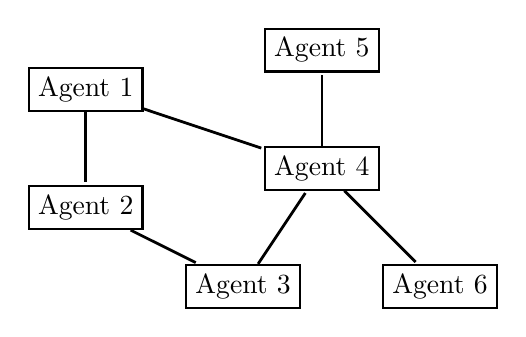
\begin{tikzpicture}
[->,>=stealth',shorten >=1pt,auto,node distance=3cm,
                    thick,main node/.style={draw}]

  \node[main node] (1) at (0, 3)  {Agent $1$};
  \node[main node] (2) at (0, 1.5)  {Agent $2$};
  \node[main node] (3) at (2, 0.5)  {Agent $3$};
  \node[main node] (4) at (3, 2)  {Agent $4$};
  \node[main node] (5) at (3, 3.5)  {Agent $5$};
  \node[main node] (6) at (4.5, 0.5)  {Agent $6$};

  \path[line width=1pt,-]
    (1) edge node {} (2)
    (1) edge node [right] {} (4)
    (2) edge node [right]{} (3)
    (3) edge node {} (4)
    (4) edge node {} (5)
    (4) edge node {} (6);
\end{tikzpicture}
\end{center}

A node represents a computational agent that stores data and performs computation, and an edge $\{i,j\}$ represents a direct connection between $i$ and $j$ through which agents $i$ and $j$ can communicate.
\end{frame}




\begin{frame}
% \frametitle{Networks and graphs}
%The word pairs (network, graph), (agent, node), and (connection, edge) are roughly synonymous.
%We use the the words \emph{network}, \emph{agent}, and \emph{connection} to refer to the physical infrastructure and \emph{graph}, \emph{node}, and \emph{edge} to refer to their corresponding mathematical abstractions.
If $\{i,j\}\in E$, then we say $j$ is adjacent to $i$ and that $j$ is a neighbor of $i$  (and vice-versa).
Write
\[
N_i=\{j\in V\,|\,\{i,j\}\in E\}
\]
for the set of neighbors $i$ and $|N_i|$ for the number of neighbors of $i$.

\vspace{0.2in}


Using the notation of graphs, we can recast problem~\eqref{eq:dist-main-opt} into
\begin{equation}
\begin{array}{ll}
\underset{\{x_i\}_{i\in V}\subset\RR^p}{\mbox{minimize}} &\displaystyle{\sum_{i\in V} \left(f_i(x_i)+h_i(x_i)\right)}\\
\mbox{subject to}&x_i=x_j\quad \forall~\{i,j\}\in E.
\end{array} \label{eq:cons_basic_prob_cons}
\end{equation}
\end{frame}



\begin{frame}
\frametitle{Why decentralized optimization?}
In a connected network, all agents can communicate with each other.
%(Any computer can communicate with any other computer over the internet.)
Any optimization method can be executed over the network through relayed communication over multiple edges.

\vspace{0.2in}

However, in distributed optimization, communication tends to be the bottleneck.
% and relayed communication incurs a huge communication cost.
So we consider algorithms that communicate across single edges 
\begin{itemize}
    \item without directly relying on long-range relayed communication,
    \item without creating a bottleneck by communicating with a single central node.
\end{itemize}
Not delegating any agent as the central agent also improves reliability against agent failure and helps data privacy.

%Therefore, methods with reduced communication costs are preferred, and


\end{frame}

\begin{frame}
\frametitle{Decentralized ADMM}
Consider $h_1=\dots=h_n=0$.
For $e=\{i,j\}$,
% introduce a variable $y_e\in\reals^p$ and
replace the constraint $x_i=x_j$ 
%of \eqref{eq:cons_basic_prob_cons} with the two constraints
with  $x_i=y_e$ and $x_j=y_e$ to obtain the equivalent problem
\[
\begin{array}{ll}
\underset{\substack{\{x_i\}_{i\in V}\\\{y_e\}_{e\in E}}}{\mbox{minimize}} &\displaystyle{\sum_{i\in V} f_i(x_i)}\\
\mbox{subject to}&
  \begin{cases}
  x_i-y_e=0\\
  x_j-y_e=0
  \end{cases} \quad \forall~e=\{i,j\}\in E.
\end{array}
\]
For each $e=\{i,j\}\in E$, introduce the dual variables  $u_{e,i}$ for $x_i-y_e=0$ and $u_{e,j}$ for $x_j-y_e=0$. The augmented Lagrangian is
\begin{align*}
\lagrange_\alpha (x,y,u)=\sum_{i}f_i(x_i)&+\sum_{e=\{i,j\}}\left(\langle u_{e,i} , x_i-y_e\rangle+\langle u_{e,j} , x_j-y_e\rangle\right)\\
&\quad +\sum_{e=\{i,j\}}\frac{\alpha}{2}\left(\|x_i-y_e\|^2+\|x_j-y_e\|^2\right).
\end{align*}
%For each agent $i$, define the set of its adjacent agents:
%\begin{align*}
%    N_i = \{\{i,j\}\in E: j\neq i\}.
%\end{align*}
%where $\sum_{e=\{i,j\}}$ is summation over all edges $e=\{i,j\}$.
\end{frame}


\begin{frame}[fragile]
% \frametitle{Decentralized ADMM}
Apply ADMM and obtain
\begingroup\makeatletter\def\f@size{9}\check@mathfonts
\begin{align*}
 \!\!\!\!\! x_i^{k+1} & = \argmin_{x_i\in \reals^p}\left\{ f_i(x_i) + \sum_{j\in N_i}\left(\langle u_{\{i,j\},i}^k,x_i-y_{\{i,j\}}^k\rangle+\frac{\alpha}{2}\|x_i-y_{\{i,j\}}^k\|^2\right)\right\}\,\,\forall i\in V\\
  \!\!\!\!\!y_e^{k+1} & = \argmin_{y_e\in \reals^p}\left\{\sum_{t=i,j} \left(\langle u_{e,t}^k, x_t^{k+1}-y_e\rangle+\frac{\alpha}{2}\|x_t^{k+1}-y_e\|^2\right)\right\}\quad\forall e=\{i,j\}\in E\\
  \!\!\!\!\!u_{e,t}^{k+1} & = u_{e,t}^k + \alpha(x_t^{k+1}-y_e^{k+1}) \qquad \forall e=\{i,j\}\in E,~t=i,j.
\end{align*}
\endgroup
%As is, this method can be implemented in a decentralized manner.
We simplify further.
\end{frame}


\begin{frame}[fragile]
% \frametitle{Decentralized ADMM}
Substitute $y_e^{k+1}=\frac{1}{2}\sum_{t=i,j}(x_t^{k+1}+\frac{1}{\alpha}u_{e,t}^k)$:
% first and third steps, thus eliminating all the $y$ components, gives us
\begin{align*}
    % x_i^{k+1} & \in \argmin_{x_i} f_i(x_i) + \frac{\alpha}{2}\sum_{j\in N_i}\left\|x_i - \frac{1}{2}\sum_{t=i,j}(x_t^{k}+\frac{1}{\alpha}u_{e,t}^{k-1}) +\frac{1}{\alpha}u_{\{i,j\},i}^k\right\|^2,\quad\forall i\in V
    % \\
    u_{e,i}^{k+1} & = u_{e,i}^k + \alpha\left(x_i^{k+1}-\frac{1}{2}\sum_{t=i,j}\left(x_t^{k+1}+\frac{1}{\alpha}u_{e,t}^k\right)\right)\\
    & = \frac{1}{2}(u_{e,i}^k-u_{e,j}^k) + \frac{\alpha}{2}(x_i^{k+1} - x_j^{k+1}), \quad \forall e=\{i,j\}\in E.
\end{align*}
Using $u_{e,i}^k+u_{e,j}^k=0$ for all $e=\{i,j\}$ and $k=1,2,\dots$,
write $y_e^{k}=\frac{1}{2}(x_i^k+x_j^k)$, $u_{e,i}^{k+1} = u_{e,i}^k + \frac{\alpha}{2}(x_i^{k+1}-x_j^{k+1})$, and
\begingroup\makeatletter\def\f@size{9}\check@mathfonts
\begin{align*}
    x_i^{k+1} & = \argmin_{x_i\in \reals^p} \left\{f_i(x_i) + \frac{\alpha}{2}\sum_{j\in N_i}\left\|x_i - \frac{1}{2}(x_i^k+x_j^k) +\frac{1}{\alpha}u_{\{i,j\},i}^k\right\|^2\right\} \\
    & = \argmin_{x_i\in \reals^p}\left\{ f_i(x_i) + \frac{\alpha|N_i|}{2}\left\|x_i - \frac{1}{|N_i|}\sum_{j\in N_i}\left(\frac{1}{2}(x_i^k+x_j^k) -\frac{1}{\alpha}u_{\{i,j\},i}^k\right)\right\|^2\right\}
\end{align*}
\endgroup
for all $i\in V$.
\end{frame}


\begin{frame}
% \frametitle{Decentralized ADMM}
Defining $v_i^k = \frac{1}{|N_i|}\sum_{j\in N_i}\left(\frac{1}{2}(x_i^k+x_j^k) -\frac{1}{\alpha}u_{\{i,j\},i}^k\right)$ and $a_i^k = \frac{1}{|N_i|}\sum_{j\in N_i}x_j^{k}$ and obtain: for every $i \in V$
\begin{align*}
     x_i^{k+1} &= \prox_{(\alpha|N_i|)^{-1}f_i(x_i)}(v_i^k) \\%&& i\in V  \\
      a_i^{k+1} &= \frac{1}{|N_i|}\sum_{j\in N_i}x_j^{k+1} \\
     v_i^{k+1} &= v_i^k + a_i^{k+1}-\frac{1}{2}a_i^k - \frac{1}{2}x_i^k%     && i\in V. \label{eq:DecenADMM_av}
  %\end{array}
\end{align*}
for $i\in V$.
%\begin{subequations}\label{eq:DecenADMM}
%\begin{align}
%%     x_i^{k+1} = \argmin_{x_i} f_i(x_i) +\frac{\alpha|N_i|}{2}\left\|x_i - v_i^k\right\|^2\\
%  %\begin{array}{ll}
%     &\,\,\,\,\,x_i^{k+1} = \prox_{(\alpha|N_i|)^{-1}f_i(x_i)}(v_i^k) && i\in V   \label{eq:DecenADMM_x}\\
%     &\begin{cases}
%      a_i^{k+1} = \frac{1}{|N_i|}\sum_{j\in N_i}x_j^{k+1} \\
%     v_i^{k+1} = v_i^k + a_i^{k+1}-\frac{1}{2}a_i^k - \frac{1}{2}x_i^k
%     \end{cases}
%     && i\in V. \label{eq:DecenADMM_av}
%  %\end{array}
%\end{align}
%\end{subequations}
This is \emph{decentralized ADMM}. Convergence follows from  convergence of ADMM.

%In step 2, each agent $i$ collects the sum of $x_j$ from its neighbors $j\in N_i$.

%Step \eqref{eq:DecenADMM_x} must be completed for all $i\in V$ before steps \eqref{eq:DecenADMM_av} start for any $i$. The two steps in \eqref{eq:DecenADMM_av} must be sequential at each $i$ but can be out of sync across different $i$.%, and Step \eqref{eq:DecenADMM_v} must be done for all $i\in V$ before the next iteration starts.
\end{frame}




\begin{frame}
% \frametitle{Decentralized ADMM}
Decentralized ADMM
\begin{align*}
     x_i^{k+1} &= \prox_{(\alpha|N_i|)^{-1}f_i(x_i)}(v_i^k) \\%&& i\in V  \\
      a_i^{k+1} &= \frac{1}{|N_i|}\sum_{j\in N_i}x_j^{k+1} \\
     v_i^{k+1} &= v_i^k + a_i^{k+1}-\frac{1}{2}a_i^k - \frac{1}{2}x_i^k%     && i\in V. \label{eq:DecenADMM_av}
  %\end{array}
\end{align*}
is decentralized:
\begin{itemize}
\item[(i)] Each agent independently performs the $x^{k+1}$- and $v^{k+1}$-updates with local computation. 
\item[(ii)] Agents send $x^{k+1}_i$ to its neighbors and each agent computes $a^{k+1}_i$ by averaging the $x^{k+1}_j$'s received from its neighbors (reduction operation in the neighborhood).
\end{itemize}
\end{frame}


\begin{frame}
\frametitle{Synchronization}
The above decentralized methods are synchronous, which can be an unrealistic requirement.
% in the sense that all agents must complete their computation and communication for the iteration to proceed.
%In some real-world decentralized networks, however, synchronization is a costly and unrealistic requirement.
\vspace{0.2in}


One can use asynchronous decentralized methods, which combine the asynchrony of \S6 with the methods of this section.
\end{frame}





\section{Decentralized optimization with mixing matrices}
\begin{frame}[plain,fragile]
\frametitle{Decentralized notation}
%We notation additional decentralized notation.
Define stack operator and use boldface to denote stacked variables:
%For notational  conciseness, we aggregate all local vectors $x_i$ as rows to define% $x_1^\intercal,\dots,x_n^\intercal$ into the matrix
\begin{align*}
  \vx = \mathrm{stack}(x_1,\dots,x_n) = \begin{bmatrix}
         \text{---}~x_{1}^\intercal~\text{---} \\
         \vdots \\
         \text{---}~x_{n}^\intercal~\text{---}
       \end{bmatrix}\in \reals^{n\times p}.
\end{align*}
%Write $\vx^k=\mathrm{stack}(x_1^k,\dots,x_n^k)$ and likewise to denote the iterates.
Write $x^\star\in\reals^p$ and $\vx^\star=\mathrm{stack}(x^\star,\dots,x^\star)\in\reals^{n\times p}$ for the solution.\\
For $\vx = \mathrm{stack}(x_1,\dots,x_n)$ and $\vy = \mathrm{stack}(y_1,\dots,y_n)$, define
\[
\langle \vx,\vy\rangle=\sum^n_{i=1}\langle x_i,y_i\rangle.
\]
For $A\succeq 0$, define $\|\vx\|_A^2=\langle \vx,A\vx\rangle$. Specifically, $\|\vx\|^2=\|\vx\|_I^2=\langle \vx,\vx\rangle$.
\end{frame}

\begin{frame}[plain,fragile]
% \frametitle{Decentralized notation}
Define
\begin{gather*}
f(\vx)=\sum_{i=1}^n  f_i(x_i),\qquad
h(\vx)=\sum_{i=1}^n  h_i(x_i)\\
\prox_{\alpha f}(\vx)=\mathrm{stack}(\prox_{\alpha f_1}(x_1),\dots,\prox_{\alpha f_n}(x_n))\\[3pt]
\nabla h(\vx)=\mathrm{stack}(\nabla h_1(x_1),\dots,\nabla h_n(x_n)).
\end{gather*}

\vspace{0.2in}

We say $\vx = \mathrm{stack}(x_1,\dots,x_n)$ is \emph{in consensus} if $x_1=\cdots=x_n$.\\
Any feasible point of \eqref{eq:cons_basic_prob_cons} is in consensus.
The methods of this section produce iterates that are in consensus in the limit.
%In other words, with sufficiently many iterations, the iterates should be in consensus approximately.
\end{frame}


\begin{frame}
\frametitle{Mixing matrices}
Informally, $W\in \reals^{n\times n}$ is a mixing matrix when an application of $W$ represents a round of communication and the aggregation of the communicated information.
Write $\lambda_1,\dots,\lambda_n$ for the eigenvalues of $W$.
%{\color{blue} Do we need to assume $\lambda_i$'s are sorted by magnitude as this sorting is used below.}
%{\color{red} Magnitude sorting is a bit awkward since sometimes sometimes we want to sort by absolute value and sometimes we want to sort by raw value when $W$ is symmetric.}

\vspace{0.2in}

$W$ is a decentralized mixing matrix with respect to $G=(V,E)$ if $W_{ij} = 0$ when $i\ne j$ and $\{i,j\}\notin E$. ($W_{ii}$ may be nonzero. $W_{ij}$ may be nonzero only if $i$ and $j$ are directly linked.)
%Consider the setup where agents $1,\dots,n$ each have access to the entries $y_1,\dots,y_n$ of the vector $y\in\reals^n$ and we wish to evaluate the 
\vspace{0.2in}

$Wy$ can be evaluated in a decentralized manner if $W$ is decentralized
\[
(Wy)_{i}=\sum^n_{i=1}W_{ij}y_j=\sum_{j\in N_i\cup\{i\}}W_{ij}y_j.
\]
\end{frame}





\begin{frame}
\frametitle{Example: Local averaging matrix}
With mixing matrix
\[
W_{i,j}=
\left\{
\begin{array}{ll}
%1&\text{ if }i=j\\
\frac{1}{|Ni|}&\text{ if }\{i,j\}\in E\\
0&\text{otherwise}
\end{array}
\right.
\]
for $i,j\in \{1,\dots,n\}$ and
\[
\tilde{f}(\vx)=\sum^n_{i=1}\frac{1}{|N_i|}f_i(x_i),
\]
we can express decentralized ADMM as
\begin{align*}
     \vx^{k+1} &= \prox_{\alpha \tilde{f}}(\vv^k)\\
     \va^{k+1} &= W\vx^{k+1}\\
     \vv^{k+1} &= \vv^k + \va^{k+1}-\frac{1}{2}\va^k - \frac{1}{2}\vx^k.
\end{align*}
%$W\vone=\vone$, however it does not satisfy the other conditions. However, $|\lambda_1(U)|=|\lambda_2(U)|=1$ is possible.
\end{frame}


\begin{frame}
\frametitle{Example: Decentralized averaging}
Agent $i\in V$ has a vector $x_i\in\RR^p$. The goal is to compute the average $\bar{x} = \frac{1}{n}\sum_{i=1}^{n} x_i$ in a decentralized manner.\\
(This is a special case of \eqref{eq:dist-main-opt} with $f_i(x)=\frac{1}{2}\|x - x_i\|^2$.)
% the solution is $\bar{x}$.
\vspace{0.2in}

Decentralized averaging method:
\[
  \vx^{k+1}= W \vx^k
\]
with the starting point $\vx^0=\mathrm{stack}(x_1,\dots,x_n)$ and a decentralized mixing matrix $W\in \reals^{n\times n}$.
\medskip

Converges to $\bar{\vx}=\mathrm{stack}(\bar{x},\dots,\bar{x})$ for all $\vx^0$ if and only if $W\vone = \vone$, $\vone^\intercal W = \vone^\intercal$, and $1=|\lambda_1| > |\lambda_2| \ge \dots \ge |\lambda_n|$. (See \ Exercise~11.4)
% {\color{blue} We allow complex eigenvalues and let $|\cdot|$ denote complex modulus. Since we must have $|\lambda_1(W)|$ as an eigenvalue of algebraic multiplicity 1, it must be real so we can write it without the modulus.}
\medskip

Condition $W\vone = \vone$ implies $\vx$-vectors in consensus are fixed points.\\
Condition $\vone^\intercal W = \vone^\intercal$ implies mean is preserved throughout the iteration.
The eigenvalue condition implies the iteration converges.
%To clarify, $|\lambda_i|$ denotes the absolute value or modulus of the $i$th\nobreakdash-eigenvalue of $W$, sorted by absolute value.
%Also, $\lambda_1$ is real, i.e., $1=\lambda_1$, since $W\vone = \vone$ and $\vone^\intercal W = \vone^\intercal$ imply that $1$ is an eigenvalue of $W$.
\end{frame}


\begin{frame}
\frametitle{Assumptions on mixing matrices}
A mixing matrix $W\in \reals^{n\times n}$ used in decentralized optimization often satisfies some or all of the following assumptions:
\begin{subequations}\label{assump:mixing_matrices}
  \begin{align}
    & W=W^\intercal \label{assump:mixing_matrices_1}\\
    & \mathcal{N}(I-W)=\mathrm{span}(\vone) \label{assump:mixing_matrices_2}\\
    & 1=|\lambda_1|>\max{\{|\lambda_2|,\dots,|\lambda_n|\}}.\label{assump:mixing_matrices_3}
  \end{align}
\end{subequations}
%\begin{itemize}
%\item [(i)]
%$W=W^\intercal$
%\item [(ii)]
% $\mathcal{N}(I-W)=\mathrm{span}(\vone)$
%\item [(iii)]
%$1=|\lambda_1|>\max{\{|\lambda_2|,\dots,|\lambda_n|\}}$.
%\end{itemize}
%where $\lambda_1,\dots,\lambda_n$ are the eigenvalues of $W$.

\vspace{0.2in}


\eqref{assump:mixing_matrices_1} was not assumed in decentralized ADMM or averaging, but it is common; methods with symmetric $W$ tend to be easier to analyze.

\eqref{assump:mixing_matrices_2} implies $\vx$ is in consensus if and only if $\vx=W\vx$ and is required for almost all decentralized optimization methods.
%For example, the local averaging matrix of decentralized ADMM
%only satisfies assumption %(ii)
%\eqref{assump:mixing_matrices_2} but not %(i) or (iii).
%\eqref{assump:mixing_matrices_1} or \eqref{assump:mixing_matrices_3}.

\eqref{assump:mixing_matrices_3} is assumed to establish the convergence of certain methods.
Note that 
\eqref{assump:mixing_matrices_1} implies the eigenvalues are real.
\end{frame}



\begin{frame}
\frametitle{Example: Laplacian-based mixing matrix}
The mixing matrix
\[
W=I-\frac{1}{\tau}L\in \reals^{n\times n}
\]
where $L$ is the so-called graph Laplacian defined by
\[
L_{i,j}=\left\{
\begin{array}{ll}
|N_i|&\text{if }{i=j}\\
-1&\text{if }{\{i,j\}\in E}\\
0&\text{otherwise}
\end{array}
\right.
\]
for $i,j\in \{1,\dots,n\}$ and $\tau$ is a constant satisfying $\tau>\frac{1}{2}\lambda_\mathrm{max}(L)$ satisfies $W=W^\intercal$, $W\vone=\vone$, and $1=\lambda_1>\max{\{|\lambda_2|,\dots,|\lambda_n|\}}$.
%See Exercise~\ref{exercise:laplacian-mixing-matrix}.
\end{frame}

\begin{frame}
\frametitle{Example: Metropolis mixing matrix}
The mixing matrix 
\[
W_{i,j}=\left\{
\begin{array}{ll}
\frac{1}{\max\{|N_i|,|N_j|\}+\varepsilon}&\text{if }\{i,j\}\in E\\
1-\sum_{j\in N_i}W_{i,j}&\text{if }{i=j}\\
0&\text{otherwise}
\end{array}
\right.
\]
for $i,j\in \{1,\dots,n\}$ and $\varepsilon>0$ satisfies $W=W^\intercal$, $W\vone=\vone$, and $1=\lambda_1>\max{\{|\lambda_2|,\dots,|\lambda_n|\}}$.
%See Exercise~\ref{exercise:metropolis-mixing-matrix}.
\end{frame}


\begin{frame}
\frametitle{Relationship with stochastic matrices}
 $P\in \reals^{n\times n}$ satisfying $P_{ij}\ge 0$  $\forall\,i,j$ and $P\vone=\vone$ is a stochastic matrix.
Mixing matrices and stochastic matrices share some apparent similarities, but they do have some key differences.
%Given a Markov chain with states $1,\dots,n$, its stochastic matrix $P\in \reals^{n\times n}$ contains the transition probabilities as $P_{ij}$ being the probability of transitioning from $i$ to $j$ for all states $i$ and $j$.


\medskip

One difference is that mixing matrices can have negative entries. 
(Cf.\ Exercise~11.16.)


\medskip

Another difference is in their primary use as linear operators.
With a stochastic matrix $P$ satisfying $P\vone=\vone$ (total probability mass of $1$ is preserved) the key operation is the vector-matrix product
\[
(\pi^{k+1})^\intercal=(\pi^k)^\intercal P.
\]
With mixing matrix $W$ satisfying $W\vone=\vone$ (vector in consensus remains in consensus) the key operation is the matrix-(stacked vector) product
\[
\vx^{k+1}=W\vx^k.
\]
\end{frame}


\begin{frame}
% \frametitle{Relationship with stochastic matrices}
When a mixing matrix is a stochastic matrix, one can utilize the classical Markov chain theory based on the Perron--Frobenius theorem.
For example, if $W\in \reals^{n\times n}$ is a stochastic matrix for an irreducible Markov chain, then $\mathcal{N}(I-W)=\mathrm{span}(\vone)$ holds; if the Markov chain is irreducible and aperiodic, then $1=\lambda_1>\max\{|\lambda_2|,\dots,|\lambda_n|\}$ holds.

\vspace{0.2in}
A Markov chain is irreducible if every state can be reached from every other state. A state of a Markov chain is periodic if the chain can return to the state only at multiples of some integer larger than 1. A Markov chain is aperiodic if none of its states is periodic.
\end{frame}

%% I removed the slide of dynamic mixing matrix since we have removed the corresponding exercise

% \begin{frame}{Dynamic mixing matrix}
% We assume the mixing matrix, once given, is fixed and do not change with iteration. It is possible however, to use a series of dynamic mixing matrices.
% \vspace{0.2in}

% Even when the graph is fixed, dynamic mixing matrices can be used to get faster convergence.
% It is possible to compute a decentralized average in $\log_2(n)$ steps using so-called exponential-2 dynamic mixing matrices. This is impossible with a fixed mixing matrix (unless the graph is complete.) See Exercises 11.X.

% \end{frame}



\begin{frame}
\frametitle{Inexact decentralized methods (using a mixing matrix)}
Consider the setup with $f_1=\dots=f_n=0$ and a mixing matrix $W\in \reals^{n\times n}$ satisfying $W=W^\intercal$, $\mathcal{N}(I-W)=\mathrm{span}(\vone)$, and $\lambda_1>\max{\{\lambda_2,\dots,\lambda_n\}}$.
We write \eqref{eq:dist-main-opt} equivalently as
\begin{equation}
\begin{array}{ll}
\underset{\vx\in\reals^{n\times p}}{\mbox{minimize}} &h(\vx)\\
\mbox{subject to}&(I-W)\vx=0.
\end{array}
\label{eq:formulation-without-penalty}
\end{equation}

\vspace{0.2in}
We consider inexact decentralized methods, DGD and Diffusion, which solve penalty formulations that approximate \eqref{eq:formulation-without-penalty}.
These inexact methods, when they converge, converge to an approximation solution.
\end{frame}





\begin{frame}
\frametitle{Decentralized gradient descent (DGD)}
Consider the penalty formulation
\[
\begin{array}{ll}
\underset{\vx\in\reals^{n\times p}}{\mbox{minimize}} &\displaystyle{h(\vx) + \frac{1}{2\alpha }\|\vx\|^2_{I-W}}.
\end{array}
\]
%Since $\|\vx\|^2_{I-W}$ equals $0$ if and only if $\vx$ is in consensus,
We expect this formulation to approximate \eqref{eq:formulation-without-penalty} well when $\alpha>0$ is small.
%(See Exercise~\ref{exercise:consensus_matrix_condition}.)
\vspace{0.2in}

Gradient descent with stepsize $\alpha$ applied to this penalty formulation is
\begin{align*}
   \vx^{k+1} & = \vx^k -\alpha \left(h(\vx^k)+\frac{1}{\alpha}(I-W)\vx^k\right)\\
   & = W\vx^k - \alpha \nabla h(\vx^k).
%   \numberthis \label{eq:dgd_itr}
\end{align*}
This is decentralized gradient descent (DGD) or the combine-then-adapt method. 
%DGD is decentralized when $W$ is a decentralized mixing matrix:
%computing $W\vx^k$ requires communication with neighbors and all other operations require local computation.
If the penalty formulation has a solution, $h_1,\dots,h_n$ are $L_h$-smooth, and $\alpha \in (0,(1+\lambda_n(W))/L_h)$, then $\vx^k$ converges to a solution of the penalty formulation.
%The stepsize bound of $(1+\lambda_n(W))/L_h$ follows from the stepsize requirement $\text{(stepsize)}\times\text{(Lipschitz-constant)}<2$ of gradient descent.
\end{frame}





\begin{frame}
\frametitle{Diffusion}
Further assume $W\succ 0$ and consider the penalty formulation
\[
\begin{array}{ll}
\underset{\vx\in\reals^{n\times p}}{\mbox{minimize}} &\displaystyle{h(\vx) + \frac{1}{2\alpha}\|\vx\|^2_{W^{-1}-I}}.
\end{array}
\]
Variable metric gradient descent \S2.8 with $\alpha^{-1} W^{-1}$ as the metric is
\begin{align*}
\vx^{k+1}  &=
\vx^k-\alpha W\left( \nabla h(\vx^k)-\frac{1}{\alpha}(W^{-1}-I)(\vx^k)\right)
\\
&= W(\vx^k - \alpha \nabla h(\vx^k)).
\end{align*}
This is the method of diffusion or the adapt-then-combine method.
%Diffusion is also decentralized when $W$ is a decentralized mixing matrix.
If the penalty formulation has a solution, $h_1,\dots,h_n$ are $L_h$-smooth, and $\alpha \in (0,2/L_h)$, then $\vx^k$ converges to a solution of the penalty formulation.
%(Exercise~11.X.)
%\begin{align*}
%\vx^{k+1} & = \vx^k - W\nabla H(\vx^k)\\
%& = W(\vx^k - \alpha \nabla h(\vx^k)).
%\numberthis\label{eq:diffusion_itr}
%\end{align*}
%Note that $W^{-1}$ appears in the analysis and formulation of the algorithm, but not within the algorithm itself.


%Given the metric matrix $M=M^\intercal\succ 0$, gradient descent under the metric $\|\cdot\|_M$ is the iteration
%\begin{align*}
%  \vx^{k+1} & = \argmin_\vx \langle \nabla H(\vx^k), x\rangle + \frac{1}{2}\|\vx - \vx^k\|^2_M\\
%  & = \vx^k - M^{-1}\nabla H(\vx^k).
%\end{align*}

%Since we wish to use $W$ rather than $W^{-1}$ in the iteration, we cannot directly apply gradient descent. Instead, we use variable metric gradient descent.

\end{frame}



\begin{frame}
\frametitle{DGD vs.\ Diffusion}
Advantages of diffusion:
\begin{itemize}
\item
Diffusion allows larger stepsizes, which often leads to faster convergence.
% \item
% Solutions to the penalty formulation of diffusion better approximate solutions to the original problem \eqref{eq:formulation-without-penalty} then those of DGD.
%If \eqref{eq:formulation-without-penalty} has a solution, the penalty formulations have solutions, but these solutions are not necessarily in consensus.
%See Exercise~\ref{exercise:original-sol-penalty-sol}.
%For the same value of $\alpha$, solutions to the diffusion penalty formulation are more in consensus than the solutions to the DGD penalty formulation and, therefore, better approximate the solution.
% See Exercises 11.X and 11.X.

%~\ref{exercise:original-sol-penalty-sol} and \ref{exercise:sol_DGD_v_Diffusion}.
%See Exercises~\ref{exercise:original-sol-penalty-sol} and \ref{exercise:sol_DGD_v_Diffusion}.
\end{itemize}

\vspace{0.2in}
Advantages of DGD:
\begin{itemize}
\item
Does not require the additional assumption $W\succ 0$; $W\vx^k$ and $\alpha \nabla h(\vx^k)$ can be computed simultaneously.
\end{itemize}

\vspace{0.2in}

When $W\nsucc 0$, we can still use diffusion with $(1-\theta) I+\theta W$ and $\theta\in(0,1/(1-\lambda_\mathrm{min}(W)))$. Since $\lambda_\mathrm{min}(W)>-1$, $\theta=\frac{1}{2}$ always works.
\end{frame}


%% Simplify the slide by removing \widetilde{W} to be consistent with the textbook

% \begin{frame}
% \frametitle{Exact decentralized methods}
% Consider two symmetric mixing matrices $W,\widetilde{W}\in\reals^{n\times n}$ satisfying
% \begin{align*}
%  & W \preceq \widetilde{W} \preceq\frac{1}{2}(I+W),\\
% %&(\widetilde{W}-W)\vx=0~\Leftrightarrow~(I-W)\vx = 0~\Leftrightarrow~x_1=\dots=x_n.
% &\mathcal{N}(\widetilde{W}-W)=\mathcal{N}(I-W)=\mathrm{span}(\vone).
% \end{align*}
% $\widetilde{W} = \frac{1}{2}(W+I)$ is a common choice.
% Since $\widetilde{W}-W\succeq 0$, there exists a symmetric $U\in\reals^{n\times n}$ such that
% \begin{align*}
%     U^2 = \widetilde{W}-W,
% \end{align*}
% and $U$ satisfies $\mathcal{N}(U)=\mathrm{span}(\vone)$.

% Consider the general problem \eqref{eq:dist-main-opt}, which is equivalent to
% \[
% \begin{array}{ll}
% \underset{\vx\in\reals^{n\times p}}{\mbox{minimize}} &f(\vx)+h(\vx)\\
% \mbox{subject to}&U\vx=0.
% \end{array}
% \]

% \end{frame}


\begin{frame}
\frametitle{Exact decentralized methods (using a mixing matrix)}
Since $I-W\succeq 0$, there exists a symmetric $U\in\reals^{n\times n}$ such that
\begin{align*}
    U^2 = \frac{1}{2}(I-W).
\end{align*}
This $U$ satisfies $\mathcal{N}(U)=\mathrm{span}(\vone)$.
\medskip

The general problem \eqref{eq:dist-main-opt} is equivalent to
\begin{equation}\label{eq:equiv-form-PGEXTRA-NIDS}
  \begin{array}{ll}
    \underset{\vx\in\reals^{n\times p}}{\mbox{minimize}} &f(\vx)+h(\vx)\\
    \mbox{subject to}&U\vx=0.
  \end{array}
\end{equation}
\medskip

We present two methods, PG-EXTRA and NIDS, what converge to its exact solution. They utilize $W$, while $U$ is used only in analysis.
\end{frame}


\begin{frame}{Exercise 3.5: Condat-V\~u, the other version}
  Consider the problem
  \[
    \underset{x\in \reals^n}{\mbox{minimize}}~f(x)+h(x)+g(Ax),
  \]
  In the derivation of Condat-V\~u, if we \emph{instead} use the metric
  \[
    M=
    \begin{bmatrix}
    (1/\alpha) I &A^\intercal\\
    A &(1/\beta) I
    \end{bmatrix},
  \]
  then we get the method
  \begin{align*}
     u ^{k+1}&=
    \prox_{\beta g^*}( u ^k+\beta Ax^k)\\
    x^{k+1}&=
    \prox_{\alpha f}(x^k-\alpha A^\intercal (2u ^{k+1}-u^k)-\alpha \nabla h(x^k)).
  \end{align*}
  If total duality holds,
  $\alpha,\beta>0$, $\alpha L/2+\alpha\beta\lambda_{\max}(A^\intercal A)<1$, and $h$ is $L$-smooth,
  then $x^k\rightarrow x^\star$ and $ u ^k\rightarrow  u ^\star$.
\end{frame}

\begin{frame}{PG-EXTRA}
  Apply the last slide to \eqref{eq:equiv-form-PGEXTRA-NIDS} with $g=\delta_{0}$ (thus $\prox_{\beta g^*}=\opI$) and $A=A^\intercal=U$ to get
  \begin{align*}
    \vu^{k+1} & = \vu^k + \beta U \vx^k\\
    \vx^{k+1} &= \prox_{\alpha f}\left(\vx^k - \alpha \nabla h(\vx^k) - \alpha U(2 \vu^{k+1}-\vu^k)\right).
  \end{align*}
  Simplify the method by choosing $\beta=\alpha^{-1}$ and introduce $\vw^k=\frac{1}{\beta}U\vu^k$ to get the PG-EXTRA method:
  \begin{align*}
    \vx^{k+1} & =\prox_{\alpha f}(W\vx^k - \alpha \nabla h(\vx^k) - \vw^k)\\
    \vw^{k+1} & = \vw^k + \frac{1}{2}(I-W)\vx^k.
  \end{align*}
  (Initialize $\vx^0$
  arbitrarily and $\vw^0=0$, which voids computing $U\vu^0$)
  \medskip
  
  PG-EXTRA is decentralized when $W$ is decentralized. If total duality holds,  $0<\alpha < (1+\lambda_{\min}(W))/L$ (using $\lambda_{\max}(U^2)=\frac{1}{2}-\frac{1}{2}\lambda_{\min}(W)$), and $h_1,\dots,h_n$ are $L$-smooth, then we have $\vx^k\to\vx^\star$.
\end{frame}

%% I commented out the older PG-EXTRA slides to be consistent with the textbook

% \begin{frame}[fragile]
% \frametitle{PG-EXTRA}
% Consider the Lagrangian
% \begin{align*}
%     \lagrange(\vx,\vy)=f(\vx)+h(\vx)+\langle \vy,U\vx\rangle,
% \end{align*}
% whose saddle subdifferential is
% %\begin{align*}
% %    \begin{bmatrix}
% %          0 \\
% %          0
% %      \end{bmatrix}\in
% %      \partial\lagrange(\vx,\vy) =
% %      \begin{bmatrix}
% %        \partial_{\vx} \lagrange(\vx;\vy) \\
% %        \partial_{\vy} (-\lagrange(\vx;\vy))
% %      \end{bmatrix},
% %\end{align*}
% %which expands to
% \begin{align*}
% %\label{eq:pdspt}
% %        \begin{bmatrix}
% %          0 \\
% %          0
% %        \end{bmatrix}
% %        \in
%       \partial \lagrange(\vx,\vy) =
%         \begin{bmatrix}
%           \partial f(\vx) \\ 0
%         \end{bmatrix}
%         +
%         %\underbrace{
%         \begin{bmatrix}
%           \nabla h & 0 \\
%           0 & 0
%         \end{bmatrix}
%         \begin{bmatrix}
%           \vx \\
%           \vy
%         \end{bmatrix}
%         %}_{\opB}
%         +
%         %\underbrace{
%         \begin{bmatrix}
%           0 & U  \\
%           -U & 0
%         \end{bmatrix}
%         \begin{bmatrix}
%           \vx \\
%           \vy
%         \end{bmatrix}.
%         %}_{\opA}
%       \end{align*}
% Define
%   \begin{align*}
%       V_\eta = \eta_1(I-\widetilde{W})+\eta_2(I-W)+\eta_3U^2,
%   \end{align*}
% where $\eta_1,\eta_2,\eta_3\in \reals$ are nonnegative, and
%   \begingroup\makeatletter\def\f@size{9}\check@mathfonts 
%   \begin{align*}
% %\label{eq:pdspt1}
% \opA(\vx,\vy) =
% \underbrace{
%         \begin{bmatrix}
%           \partial f(\vx) \\ 0
%         \end{bmatrix}
% +
%         \begin{bmatrix}
%          0 & \frac{1}{2}U  \\
%           -\frac{1}{2}U & 0
%         \end{bmatrix}
%         \begin{bmatrix}
%           \vx \\
%           \vy
%         \end{bmatrix}
% }_{=\opF(\vx,\vy)}
%         +
%         \underbrace{
%         \begin{bmatrix}
%           \nabla h & 0 \\
%           0 & 0
%         \end{bmatrix}
%         \begin{bmatrix}
%           \vx \\
%           \vy
%         \end{bmatrix}
%         %}_{\opB}
%         +
%         \begin{bmatrix}
%          \alpha^{-1} V_\eta & \frac{1}{2}U  \\
%           -\frac{1}{2}U & 0
%         \end{bmatrix}
%         \begin{bmatrix}
%           \vx \\
%           \vy
%         \end{bmatrix}
% }_{=\opH(\vx,\vy)}.
% \end{align*}
% \endgroup
% Then $\zer \opA(\vx,\vy)=\zer\partial \lagrange(\vx,\vy)$, since $U\vx=0$ implies $V_\eta\vx=0$.
% We apply variable metric FBS to $\opA$, rather than $\partial \lagrange$.
% \end{frame}


% \begin{frame}[plain]
% % \frametitle{PG-EXTRA}
% The matrix
% \begin{align*}
% %      \opF = \begin{bmatrix}
% %              \partial f  & \frac{1}{2}U  \\
% %                -\frac{1}{2}U &
% %             \end{bmatrix},
% %        ~~
% %      \opH = \begin{bmatrix}
% %        \alpha^{-1}V_\eta + \nabla h & \frac{1}{2}U  \\
% %                -\frac{1}{2}U &
% %             \end{bmatrix},
% %        ~~
%       M = \begin{bmatrix}
%         \alpha^{-1}I & -\frac{1}{2}U  \\
%         -\frac{1}{2}U & \beta^{-1}I
%         \end{bmatrix}
%     \end{align*}
% satisfies $M\succ 0$ if $4I\succ \alpha\beta U^2$.
% %Then $\opF$ is maximally monotone, $\opH$ is so when $\eta\ge 0$, and $M=M^\intercal\succ 0$ when $I\succ 4\alpha\beta U  U$.
% FPI with $(M+\opF)^{-1}(M-\opH)$ is
% \begin{align*}
%     \vx^{k+1} & = \prox_{\alpha f}\big((I-V_\eta)\vx^k - \alpha \nabla h(\vx^k) - \alpha U \vy^k\big)\\
%     \vy^{k+1} & = \vy^k + \beta U\vx^{k+1}.
% \end{align*}
% We initialize $\vy^0 = \beta U\vx^0$ (but set $\vx^0$ arbitrarily).
% Let $\eta_1=1$, $\eta_2=0$, $\eta_3=0$, $\beta=1/\alpha$ and substitute $\vy^k= \sum_{i=0}^{k}U\vx^i$ to get
% %Let $\vx^{-1}=\vx^0$.
% \[
%     \vx^{k+1}  = {\prox_{\alpha f}}\left(W\vx^k-\alpha\nabla h(\vx^k) - \sum_{j=0}^{k-1}(\widetilde{W}-W)\vx^j\right).
% \]
% This is PG-EXTRA. 
% Method  is decentralized when $W$ and $\widetilde{W}$ are decentralized mixing matrices.
% If $\lagrange$ has a saddle point, $h_1,\dots,h_n$ are $L_h$-smooth, and $\alpha \in (0,2\lambda_\mathrm{min}(\widetilde{W})/L_h)$, then $\vx^k\rightarrow \vx^\star$.
% \end{frame}

\begin{frame}{Review of PD3O}
    Consider
    \[
    \begin{array}{ll}
    \underset{\vx\in\reals^{n\times p}}{\mbox{minimize}} & f(x) + h(x) + g(Ax)
    \end{array}
    \]
    where $h$ is $L$-smooth. PD3O is the method
    \begin{align*}
        x^{k+1} &= \prox_{\alpha f}\left(x^k - \alpha A^\intercal u^k - \alpha\nabla h(x^k)\right)\\
        u^{k+1} &= \prox_{\beta g^*}\left(u^k+\beta A(2x^{k+1}-x^k+\alpha\nabla h(x^k)-\alpha h(x^{k+1}))\right).
    \end{align*}
    (PD3O can be obtained by applying DYS FPI and BCV to the problem.)
    \medskip
    
    If total duality holds, $\alpha,\beta>0$, $\alpha\beta\lambda_{\max}(A^\intercal A)\le 1$, and $\alpha\le 2/L$, then $x^{k+1/2}\to x^\star$.
\end{frame}


\begin{frame}
\frametitle{NIDS}
Apply PD3O to 
\[
\begin{array}{ll}
\underset{\vx\in\reals^{n\times p}}{\mbox{minimize}} & f(\vx) + h(\vx) + \delta_{\{0\}}(U\vx).
\end{array}
\]
to get
\begin{align*}
  \vx^{k+1} & = \prox_{\alpha f}(\vx^k - \alpha U  \vu^k - \alpha \nabla h(\vx^k))\\
  \vu^{k+1} & = \vu^k + \beta U\left(2\vx^{k+1}-\vx^{k} + \alpha \left(\nabla h(\vx^k) - \nabla h(\vx^{k+1})\right)\right)
\end{align*}

\end{frame}

\begin{frame}
To eliminate $U$, define $\vz^k = \vx^k - \alpha U  \vu^k - \alpha \nabla h(\vx^k)$. Use $\beta=\alpha^{-1}$ to get
\begin{align*}
  \vx^{k+1} & = \prox_{\alpha f}(\vz^k)\\
  \vz^{k+1} & = \vz^k - \vx^{k+1} + \frac{1}{2}(I+W)\left(2\vx^{k+1}-\vx^k + \alpha \left(\nabla h(\vx^k) - \nabla h(\vx^{k+1})\right)\right)
\end{align*}
with arbitrary $\vx^0$ and $\vz^0 = \vx^0 - \alpha \nabla h(\vx^0)$. This uses $\vu^0=0$, which avoids computing $U\vx^0$.
\bigskip

This is the \emph{Network InDependent Step-size} (NIDS) method.
%NIDS is also decentralized.
If total duality holds, $h_1,\dots,h_n$ are $L_h$-smooth, and $\alpha \in(0,2/L_h)$, then $\vx^k\rightarrow \vx^\star$.
\bigskip

The choice of $\alpha\in(0,2/L_h)$ is independent of the mixing matrix and, thus, the network topology.
\end{frame}

%% the NIDS slide below was adjusted to the updated textbook

% \begin{frame}[fragile]
% % \frametitle{NIDS}
% Define $\vz^k = \vx^k - \alpha U  \vu^k - \alpha \nabla h(\vx^k)$:
%   \begingroup\makeatletter\def\f@size{9}\check@mathfonts
% \begin{align*}
% %  \label{eq:nids_x}
%   \vx^{k+1} & = \prox_{\alpha f}(\vz^k)\\
%  % \label{eq:nids_z}
%   \vz^{k+1} & = \vz^k - \vx^{k+1} + (I-\beta(\widetilde{W}-W))\left(2\vx^{k+1}-\vx^k + \alpha \left(\nabla h(\vx^k) - \nabla h(\vx^{k+1})\right)\right)
% \end{align*}
% \endgroup
% and initialize $\vz^{0} = \vx^0 - \alpha \nabla h(\vx^0)$ (but set $\vx^0$ arbitrarily).
% % and, for $k=0,1,\dots$,
% \vspace{0.2in}

% This is the Network InDependent Step-size (NIDS) method.
% %NIDS is also decentralized.
% If $\lagrange$ has a saddle point, $h_1,\dots,h_n$ are $L_h$-smooth, $\alpha \in(0,2/L_h)$ and $\beta> 0$ satisfies $I-\alpha\beta(\widetilde{W}-W)\succeq 0$, then $\vx^k\rightarrow \vx^\star$.

% \vspace{0.2in}

% By setting $\widetilde{W}= \frac{1}{2}(W+I)$ and $\beta = \alpha^{-1}$, we obtain $I-\alpha\beta(\widetilde{W}-W)=\frac{1}{2}(W+I)\succeq 0$, so the choice of $\alpha\in(0,2/L_h)$ is independent of the mixing matrix and, thus, the network topology.
% \end{frame}


\begin{frame}
\frametitle{PG-EXTRA vs\ NIDS}
The step size $\alpha$ of PG-EXTRA depends on the eigenvalues of $W$. This not only limits the size of $\alpha$ but also make the choice of $\alpha$ more difficult when the network is not fully known.
In contrast, NIDS allows the stepsize $\alpha$ to be larger and to be chosen independent of $W$.
\bigskip

On the other hand, PG-EXTRA can compute $W\vx^k$ and $\nabla h(\vx^k)$ simultaneously, but NIDS cannot.
\bigskip

%The first method, EXTRA, is easier to derive but involves a step-size parameter than depends on properties of $W$. The other, NIDS, which is slightly more complicated, has a step-size parameter that can be chosen independent of the properties of $W$.
% It is easy to see their differences under the simplification: , which yields $\prox_{\alpha f}=I$ and, in NIDS, $\vz^k = \vx^k$:
With $f= 0$ and $\widetilde{W}=\frac{1}{2}(W+I)$, the methods simplify to
\begin{align*}
\text{PG-EXTRA:}&\quad \vx^{k+1}=\widetilde{W}(2\vx^k - \vx^{k-1}) + \alpha(\nabla h(\vx^{k-1})-\nabla h(\vx^k))\\
  \text{NIDS:}&\quad  \vx^{k+1}=\widetilde{W}\left(2\vx^k - \vx^{k-1} + \alpha(\nabla h(\vx^{k-1})-\nabla h(\vx^k))\right).
\end{align*}
PG-EXTRA resembles DGD while NIDS resembles diffusion.

%See Exercise~\ref{exercise:extra_eqv_forms}.

\end{frame}

\iffalse
\begin{frame}
\frametitle{DIGing}
Let $\overline{W}\in \reals^{n\times n}$ be a mixing matrix. The method
\begin{align*}
  \vx^{k+1} & = \overline{W}\vx^k - \vz^k \\
  \vz^{k+1} & = \overline{W}\vz^k + \alpha\left(\nabla h(\vx^k) - \nabla h(\vx^{k-1})\right),
\end{align*}
is called DIGing.
DIGing is a special case of PG-EXTRA with $f=0$, $\beta=1$,  $W=2\overline{W}-I$, and $\widetilde{W}= \overline{W}\overline{W}$.
% See Exercise~\ref{exercise:diging}.

The $\vx$ update is similar to DGD \eqref{eq:dgd_itr} where $\alpha\nabla h(\vx^k)$ is replaced by $\vz^k$.
Comparing the $\vz$ update to that in Exercise \ref{exercise:tracking_in_network}, we can see $\vz^k$ trails the mean $\frac{1}{n}\sum_{i=1}^{n}\nabla h_i(x_i^k)$. Show that
{\color{red} QUESTION TO WOTAO: What does ``trail'' mean?}{\color{blue} ``track'' is a better word.}
\begin{enumerate}
  \item If $\vx^k\to\bar{\vx}$ and $\vz^k\to \frac{1}{n}\sum_{i=1}^{n}\nabla h_i(\bar{x}_i)$ for some $\bar{\vx}$, then $\bar{\vx}$ is a solution to \eqref{eq:cons_basic_h_prob};
  \item Show that DIGing is a special case of EXTRA. (Hint: let $W=2\overline{W}-I$ and $\widetilde{W}= \overline{W}\overline{W}$.)
\end{enumerate}
Therefore, if $\overline{W}$ and $\alpha$ are chosen such that the equivalent setup of EXTRA converges to a solution of \eqref{eq:cons_f_g_prob}, DIGing also does.
% Like EXTRA and unlike DGD, DIGing has ``exact convergence.''
XXX
\end{frame}

\fi 

\begin{frame}{Conclusion}
  Distributed optimization takes advantages of problem structures and can solve extremely large optimization problems.
  \bigskip
  
  With a central coordinator, the methods rely on aggregating distributed gradients or averaging distributed iterates through a reduce operation.
  \bigskip
  
  Decentralized optimization uses neighborhood communication (i.e., decentralized mixing) instead of a global reduce operation.
  \bigskip

  By applying splitting and variable metric techniques, we obtain decentralized optimization methods.
\end{frame}


\end{document}
